\documentclass[12pt,a4paper]{article}
\usepackage{tabularx}
\usepackage{booktabs}
\usepackage{longtable}
\usepackage{ltxtable}
\usepackage[latin1]{inputenc}
\usepackage{amssymb}
\usepackage[]{graphicx,rotating}
\usepackage[T1]{fontenc}
\usepackage{parskip}
\usepackage{listings}
\usepackage{natbib}
\usepackage[official]{eurosym}
\usepackage{mathrsfs}
\usepackage{amsmath}
\usepackage{verbatim}
\usepackage{epstopdf} % to include eps files
\usepackage{enumitem} % for the abbreviations table


\usepackage[usenames,dvipsnames]{color}     %for R colors and formatting
\usepackage{tikz,pgfplots,pgf}% for drawing neural net
\usepackage{neuralnetwork}
\usetikzlibrary{matrix,shapes,arrows,positioning}

\usepackage[left=3cm, right=2.5cm, top=2.5cm]{geometry}

\pagestyle{empty}
\parindent 0.0cm
\renewcommand{\baselinestretch}{1}
\newcommand{\bs}{\boldsymbol}
\renewcommand{\familydefault}{cmr} % alternative: cmss
\pdfminorversion=7
\bibliographystyle{agsm}
% for formatting packages, R, and Code
\newcommand{\pkg}[1]{{\normalfont\fontseries{b}\selectfont #1}}
\let\proglang=\textsf
\let\code=\texttt

\pgfplotsset{compat=1.16} % for backward compatibility of pgfplots package

\lstset{ %for R colors and formatting
  language=R,                     % the language of the code
  basicstyle=\scriptsize\ttfamily, % the size of the fonts that are used for the code
  numbers=left,                   % where to put the line-numbers
  numberstyle=\scriptsize\color{Blue},  % the style that is used for the line-numbers
  stepnumber=1,                   % the step between two line-numbers. If it is 1, each line
                                  % will be numbered
  numbersep=5pt,                  % how far the line-numbers are from the code
  backgroundcolor=\color{white},  % choose the background color. You must add \usepackage{color}
  showspaces=false,               % show spaces adding particular underscores
  showstringspaces=false,         % underline spaces within strings
  showtabs=false,                 % show tabs within strings adding particular underscores
  frame=single,                   % adds a frame around the code
  rulecolor=\color{black},        % if not set, the frame-color may be changed on line-breaks within not-black text (e.g. commens (green here))
  tabsize=2,                      % sets default tabsize to 2 spaces
  captionpos=b,                   % sets the caption-position to bottom
  breaklines=true,                % sets automatic line breaking
  breakatwhitespace=false,        % sets if automatic breaks should only happen at whitespace
  keywordstyle=\color{RoyalBlue},      % keyword style
  commentstyle=\color{YellowGreen},   % comment style
  stringstyle=\color{ForestGreen}      % string literal style
} 

\begin{document}

\begin{center}
% \vspace*{1cm}
 
\includegraphics[width=0.35\textwidth]{GU-Logo-blau-CMYK.eps} \vspace{2cm}
  
%  {\Large{\bf Predicting Cross-Sell with Artificial Neural Networks}} \newline
%  {\Large{An Empirical Study of ING's Customer Data}} \vspace{0.5cm}
{\large{\bf Un-Black-Boxing Artificial Neural Networks}}

{\large{Predicting and Explaining Bank Customer's Cross-Sell Likelihood}} \vspace{0.5cm}


  Seminar Thesis \\\vspace{2cm}
  submitted to \\\vspace{0.5cm}
  \textbf{Hon.-Prof. Dr. Martin Schmidberger} \\
  \textbf{Gabriela Alves Werb} \\\vspace{0.5cm}
  Goethe University Frankfurt am Main \\
  School of Business and Economics \\
  Chair for E-Commerce \vspace{2cm}
  
  by \\\vspace{0.5cm}
  \textbf{Lukas J\"urgensmeier} \\
  (Mat.-Nr.: 6904281) \\
  
  \medskip
  \medskip
  in partial fulfillment of the requirements \\
  for the degree of \\\vspace{0.5cm}
  \textbf{Master of Science in Business Administration} \\\vspace{0.5cm}
  July 15, 2019
  
\end{center}


\pagebreak
\pagestyle{plain}
\pagenumbering{Roman}
\tableofcontents
\pagebreak
\listoffigures
\listoftables
\newpage
\newlist{abbrv}{itemize}{1}
\setlist[abbrv,1]{label=,labelwidth=1in,align=parleft,itemsep=0.1\baselineskip,leftmargin=!}
 
\section*{List of Abbreviations}
%\chaptermark{List of Abbreviations}
 
\begin{abbrv}
 
\item[ANN]			Artificial Neural Network
\item[API]				Application Programming Interface
\item[AUC]			Area Under Curve
\item[LIME]			Local Interpretable Model-agnostic Explanation
\item[ReLU]			Rectified Linear Unit
\item[ROC]			Receiver Operating Characteristics
\item[SP]				Submodular Pick
 
\end{abbrv}
\newpage
\setcounter{page}{2}
\pagenumbering{arabic}
\setlength{\baselineskip}{1.5\baselineskip}
\pagestyle{plain}


\section{Introduction}

The rise of machine learning techniques has come with a great increase
of predictive accuracy in many settings \citep{jordanMachineLearningTrends2015}. The hype around those techniques has led to a widespread use of them in many fields in science and practice---from medicine to business or self-driving cars \citep{chenMachineLearningPrediction2017}.
However, some of those methods are increasingly computationally expensive and might not in every case be superior to traditional regression-based methods such as simple multivariate linear regression or logit models.

This paper uses a data set from a large German bank with numerous customer characteristics to predict whether an existing customer buys another
product---also referred to as cross-selling.
The goal of this research is first to predict weather a customer will cross-buy and open a checking account and second to identify certain characteristics of typical customers that increase the likelihood of opening that account.
Therefore, this paper introduces a complex Artificial Neural Network (ANN) with optimized predictive power and compares the predictions to a simple logit model.
One downside of ANN models in particular the lack of interpretability---they are widely regarded as black-boxes \citep{benitezAreArtificialNeural1997, dayhoffArtificialNeuralNetworks2001}.
This paper addresses this shortcoming by implementing LIME---a method to explain individual predictions of neural networks \citep{ribeiroWhyShouldTrust2016a}.
The paper is structured as follows: The first chapter gives a short introduction to cross-selling theory and is followed by the explanation of the implemented statistical methods.
The subsequent chapter presents the empirical results and especially compares the ANN to the simple logit model.
The paper concludes with implications for practitioners and outlines further research avenues.

\section{A Short Primer on Cross-Sell}
Cross-selling is an important action field for established companies with an existing customer base \citep{liCrossSellingRightProduct2011}.
Selling additional products to present customers taps into a readily accessible target group for additional sales potential.
\cite{felveyCrosssellingComputer1982} argues that a businesses' client base might already be more inclined to buy another product from the company that they already have a relationship with, compared to non-customers.
Also, the cost of selling additional products to already existing customers is cheaper than targeting new ones \citep{reichheldZeroDefectionsQuality1990}.
Benefits of cross-selling from the company point-of-view include increased switching costs for customers, while customers benefit from an easy integration
of different products and a higher certainty about the quality of the new product \citep{kamakuraApplyingLatentTrait1991, kamakuraCrosssellingDatabaseMarketing2003}. 
However, as in most business settings, there is no free lunch and hence cross-selling efforts are also associated with costs and risks.
Apart from trivial costs for cross-selling efforts such as mailing or telephone campaigns, there is a significant churn risk involved.
If not accurately targeted, customers can be annoyed by irrelevant and continuous advertisement and might eventually churn as a result \citep{keaveneyCustomerSwitchingBehavior1995}.
Due to the significant sales potential on the one hand and costs and risks involved on the other hand, it is therefore paramount to accurately identify the target group that is most likely to cross-buy another product.
This paper addresses this issue and presents an Artificial Neural Network to accomplish that task in the best possible way.


\section{Methodology}
This section provides an overview over the implemented methodology by first outlining the feature engineering process that transforms the original data set
to suitable format for neural networks.
The second part then describes the ANN and its initial architecture, while the third part describes the hyperparameter tuning process
that leads to the \textit{best} model\footnote{This model is definitely not the best model \textit{existing}, but the best model \textit{found} through the trial-and-error tuning process described in detail in section \ref{sec_crossval}.}.
Lastly, this section addresses a common criticism of machine learning technologies in general and neural networks in particular---the 
uninterpretable black box---by introducing the Local Interpretable Model-agnostic Explanation (LIME) as a method to 
"look under the hood" of a neural network and determine which features contributed by how much to a prediction.

\subsection{Feature Engineering and Data Set Preparation}
In order to feed seamlessly into a neural network, extensive feature engineering and data preparation is required \citep{hastieElementsStatisticalLearning2017}.
Before training the model, I replace missing values in \code{pref\_device} and \code{occupation} by \code{None\_or\_missing}, transform all \code{char} variables to a \code{factor} type, and remove the misleading feature \code{ID}.
However, there are still numerous features including missing values. Since they are not missing at random, they need to be imputed in order to not
bias the prediction.
Deleting all observations with missing values would do exactly that.
Hence, I impute missing values with a Random Forest from the \pkg{randomForest}\code{::rfImpute()} function.
This algorithm first replaces missing numeric (factor) variables with the median (mode) and then uses proximity measures from \code{randomForest}
as weights to replace \code{NA's} with the weighted average of the non-missing values and repeats this for a
pre-defined number of iterations\footnote{After four iterations the out-of-bag error did not decrease notably anymore, hence four iterations were chosen.}
 \citep{liawClassificationRegressionRandomForest2002}.
I furthermore bin the continuous features \code{age}, \code{entry\_age} and \code{last\_acc}\footnote{Those three features exhibit a highly
non-linear relationship. According to the universal approximation theorem, a 
neural network with enough units in a hidden layer can approximate any continuous function \citep{hornikApproximationCapabilitiesMultilayer1991}.
The best neural network will be found by trying out different hyperparameters, including some combinations which would not have \textit{enough}
hidden layer units for a solid approximation. Hence, I bin
those three variables to make sure that this non-linear relationship can be taken into account by the model in any case. Also, the benchmark logit model
could not capture this effect without further specification.}
in four distinct groups.
Since a neural network cannot handle multi-categorical features, the routine dummy-codes those.
Finally---to not distort the input weights for the first hidden layer and thus not negatively affect the prediction quality 
\citep[pp. 398]{hastieElementsStatisticalLearning2017}---I standardize all input features to exhibit $\bar{x}=0$ and $s=1$.
The feature engineered data set consists of $n_x = 74$ input variables that will be used to predict cross-sell. 
% uncommented due to page limitation
%\begin{figure}[ht]
%	\centering
%  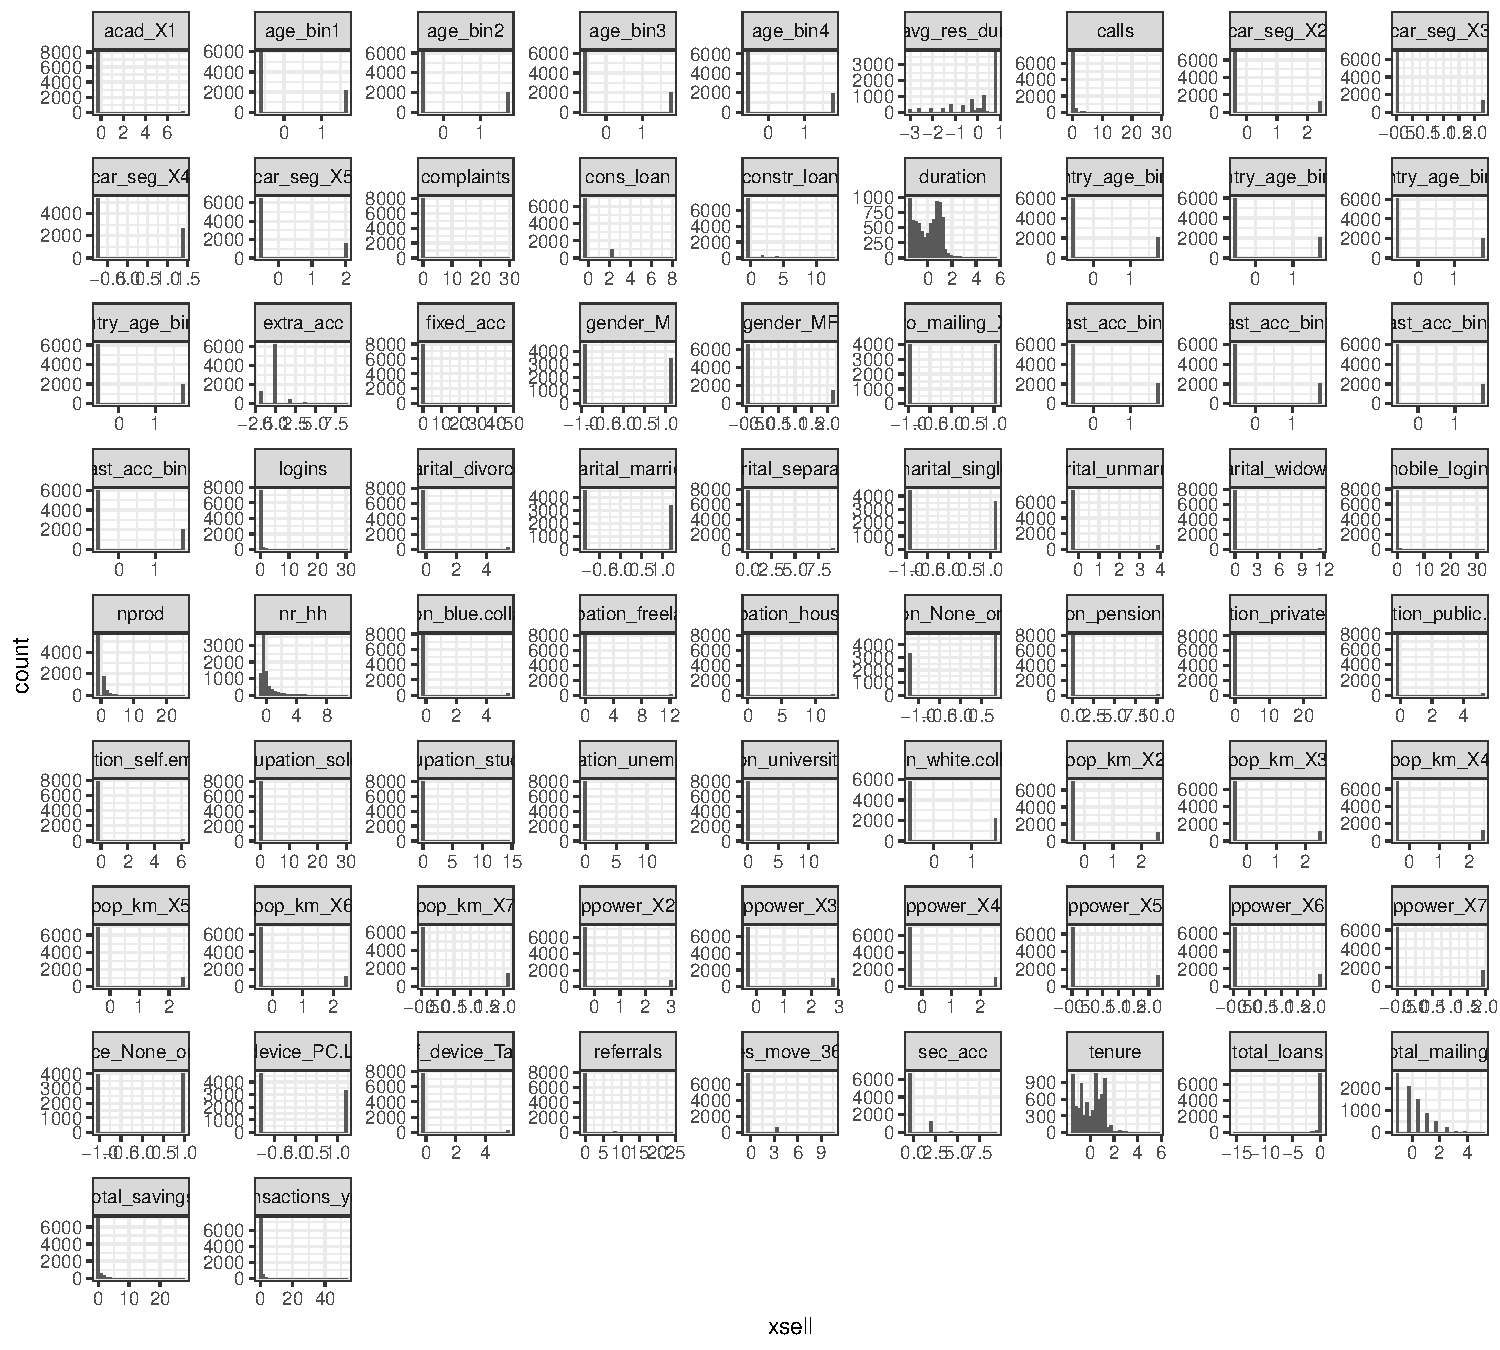
\includegraphics[scale=0.63]{figures/hist_all_features.pdf}
%	\caption{Histogram of all features after feature engineering process}
%	\label{fig_hist}
%\end{figure}Figure \ref{fig_hist} displays the histograms for each
%of those features.

\subsection{Artificial Neural Network with Keras}

While the previous section discussed the steps required to transform the data to a suitable format for an ANN,
this part describes the basic architecture of this classification method.
This study uses the \proglang{R} interface \pkg{keras} \citep{cholletInterfaceKeras2017} to the popular same name \proglang{Python} library.
As a high-level API, it enables an easier way to access the features of Google's \pkg{TensorFlow} \citep{abadiTensorFlowLargeScaleMachine2015}.

The neural network in this study is a common feedforward network which uses the backpropagation algorithm to adjust its weights \citep{werbosBackpropagationTimeWhat1990}.
Based on the feature engineering process described in the previous section, the ANN has $n_x = 74$ inputs $X_i$, 
two hidden layers with neurons $H_i^l$ referring to the $i^{th}$ neuron in the $l^{th}$ hidden layer. 
The number of neurons in the hidden layers is subject to hyperparameter tuning in the following section.
As a final layer, the ANN predicts the single binary output $\hat{Y}_i$, in our case \code{xsell}.
Figure \ref{fig_nn_arch} graphically visualizes the architecture.
\begin{figure}
\begin{center}
\def\layersep{3.5cm}

\begin{tikzpicture}[
   shorten >=1pt,->,
   draw=black!50,
    node distance=\layersep,
    every pin edge/.style={<-,shorten <=1pt},
    neuron/.style={circle,fill=black!25,minimum size=17pt,inner sep=0pt},
    input neuron/.style={neuron, fill=green!50},
    output neuron/.style={neuron, fill=red!50},
    hidden neuron/.style={neuron, fill=blue!50},
    annot/.style={text width=4em, text centered}
]

    % Draw the input layer nodes
    \foreach \name  [count=\y] in 
    {acad\_X1, age\_bin1, \dots,  age\_bin4, mobile\_logins, tenure, \dots, total\_mailings, transactions\_year}
     {   \node[input neuron, pin=left:\name] (I-\y) at (0,-\y cm) {};  
     }

    % set number of hidden layers
    \newcommand\Nhidden{2}
    \newcommand\NodOne{5}
    \newcommand\NodTwo{10}
    \newcommand\Nod{9}

    % Draw the hidden layer nodes
%    \foreach \N in {1,...,\Nhidden} {

     \foreach \y in {1,...,\NodOne} {
          \path[yshift=-1.80cm]
              node[hidden neuron] (H1-\y) at (1*\layersep,-\y cm) {};
              }
    \node[annot,above of=H1-1, node distance=2.8cm] (hl1) {Hidden layer 1};
     \foreach \y in {1,...,\NodTwo} {
          \path[yshift=0cm]
              node[hidden neuron] (H2-\y) at (2*\layersep,-\y cm) {};            
           }
    \node[annot,above of=H2-1, node distance=1cm] (hl2) {Hidden layer 2};          

%    }

    \node[below=3.2cm of H1-\NodOne] (text1) {64 neurons};
    \node at (text1 -| H2-1) (text2) {128 neurons};
	\node at (text1 -| I-9) (text1) {74 inputs};

    % Draw the output layer node
    \node[output neuron,pin={[pin edge={->}]right:xsell}, right of=H\Nhidden-5] (O) {};

    \node at (text1 -| O) (text3) {1 output};
    % Connect every node in the input layer with every node in the
    % hidden layer.
    \foreach \source in {1,...,9}{
        \foreach \dest in {1,...,\NodOne}{
            \path (I-\source) edge (H1-\dest);
         }
    }
    % connect all hidden stuff
    \foreach [remember=\N as \lastN (initially 1)] \N in {2,...,\Nhidden}
       \foreach \source in {1,...,\NodOne}
           \foreach \dest in {1,...,\NodTwo}
               \path (H\lastN-\source) edge (H\N-\dest);

    % Connect every node in the hidden layer with the output layer
    \foreach \source in {1,...,\NodTwo}
        \path (H\Nhidden-\source) edge (O);

    % Annotate the layers

    \node[annot,left of=hl1] {Input layer};
    \node[annot,right of=hl\Nhidden] {Output layer};
\end{tikzpicture}
% End of code
\label{fig_nn_arch}
\caption{Architecture of the Artificial Neural Network implemented in this study}
\end{center}
\end{figure} \label{fig_nn_arch}
This network uses a random uniform distribution $U(-0.05, 0.05)$ to initialize the weights for each neuron $H_i^l$.
Also, a bias initialized at zero feeds into the two hidden layers, for which each $H_i^l$ is activated by a rectifier function (\code{ReLU}).
\cite{glorotDeepSparseRectifier2011} show that rectifying units in an ANN yield superior outcomes compared to others such as the hyperbolic tangent activation function. Since the output $\hat{Y}_i$ is a binary feature, I use a sigmoid activation function for the output layer.
To avoid overfitting, the model implements dropout for the hidden layers.
This process randomly drops neurons and their connections from the ANN and thus leads to a more generalizable model \citep{srivastavaDropoutSimpleWay2014}.
Mitigating the risk of overfitting to the training data is furthermore a key objective of the next section.

\subsection{Cross-validation and Hyperparameter Tuning} \label{sec_crossval}
After setting up the basic architecture of the neural network, this section describes the process that leads to the \textit{best} model\footnote{as mentioned earlier, this is not the best model \textit{existing}, but \textit{found}.}.
An important feature of the \textit{best} model is that it does not memorize the exact relationships in the training data set---overfitting---but
rather learns the generalizable underlying mechanisms an thereby performs well on the holdout validation and subsequently on the test or even an out-of-time data set. 
For this purpose I first describe the optimization of the ANN by cross-validating predictions of several training epochs with a holdout 
sample and then introduce hyperparameter tuning---a process that leads to the most desirable\footnote{"Desirable" is defined as most accurate in this study. However, other metrics such as loss are also valid optimization criteria.} configuration of the ANN by
running many combinations of different model specifications.

To compile the ANN, I use the adaptive moment estimation algorithm \code{Adam} \citep{kingmaAdamMethodStochastic2014}.
\cite{ruderOverviewGradientDescent2016} recommend this gradient descent optimizer as computationally inexpensive and performing best in most applications.
This optimizer minimizes the cross-entropy loss \citep{zhangGeneralizedCrossEntropy2018} for each training epoch and accordingly updates the weights
for the next model.
Figure \ref{fig_history} shows the training history of the chosen ANN over ten epochs. The cross-entropy loss is plotted in the top pane, and the accuracy
displayed in the bottom part, each for the training and validation data set.

\begin{figure}[ht]
	\centering
  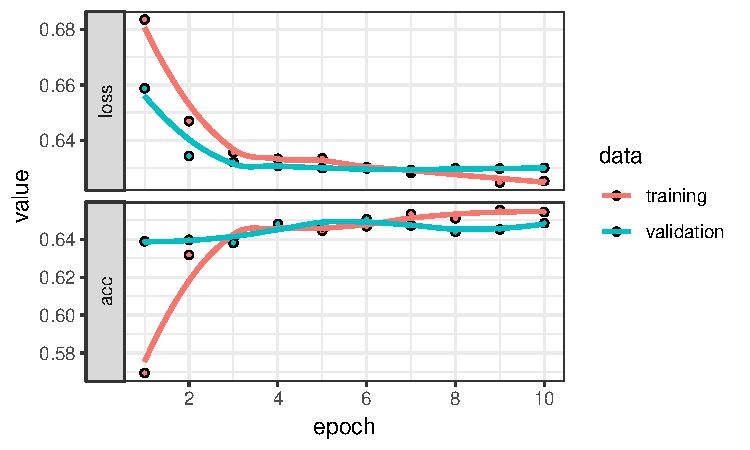
\includegraphics[scale=0.8]{figures/train_history.pdf}
	\caption{Loss and accuracy for training and test data over training history of the tuned model}
	\label{fig_history}
\end{figure}
The validation accuracy in comparison with the training accuracy in this case indicates first how accurate the ANN predicts true positives 
and true negatives in both data sets, but more importantly, gives an indication whether overfitting is an issue.
If the training accuracy kept steadily increasing, while the validation accuracy remained relatively constant, the model would overfit---which means
that the model is not generalizable beyond the training data set \citep{hansenNeuralNetworkEnsembles1990}.
As exhibited in figure \ref{fig_history}, both accuracies are relatively constant and rather similar during the last training epochs.
This is a strong indication that the model does not overfit and will perform similarly well on the test or out-of-time data.

However, one question remains unanswered with cross-validation: Which model architecture leads to the most accurate predictions?
Hyperparameter tuning provides a remedy to this issue \citep{bergstraRandomSearchHyperparameter2012}.
In short, this process runs numerous models with different combinations of hyperparameters\footnote{Hyperparameters refer to the specifications of an ANN,
such as number of units per hidden layer, dropout rate and weights, but also different optimization algorithms and activation functions \citep{bengioGradientbasedOptimizationHyperparameters2000}}. 
The model with the highest validation accuracy \code{val\_acc} is then chosen to be the \textit{best} model for predicting \code{xsell}.
This study uses the "naive" grid method, which runs all possible combinations of pre-defined values for hyperparameters\footnote{I use each three different values of the hyperparameters \code{val\_acc}, \code{acc}, \code{units1}, \code{dropout1}, \code{units2}, \code{dropout2}, \code{epochs} and \code{batch}}.
However, this method is computationally expensive.
It requires $N=a^b$ different models, where $a$ is the number of discrete values for each parameter and $b$ is the 
number of hyperparameters to be tuned.
Running two separate sets of hyperparameter combinations for 324 different models in total took roughly five hours on a standard consumer laptop.
It can be assumed that this limited set of combinations did by far not yield the best model.
However, this naive grid method runs an exponentially increasing number of different models and thus gets difficult to handle quite quickly.
A possible solution to this problem is random search, which is even more efficient than grid search \citep{bergstraRandomSearchHyperparameter2012}.

By cross-validating the predictions with a loss function and by tuning the ANN's hyperparameter, 
this section described the approach to finding the most suitable model for the prediction task at hand.
The next part turns to prediction explanation---a key discussion point and critique of neural networks.

\subsection{Local Interpretable Model-agnostic Explanation (LIME)} \label{sec_lime_theory}
In contrast to traditional regression-based methods that yield beta coefficients and enable the construction of a functional form of 
the underlying mechanisms in the data, a neural network does not provide an easily interpretable function that links $Y_i$ to $X_i$.
A common criticism of ANN hence is the "black-box" argument \citep{benitezAreArtificialNeural1997, dayhoffArtificialNeuralNetworks2001}.
Though the model might yield more accurate predictions, there is no clear answer to the question why the model predicted those particular values
or which features contributed by how much.

With the development of new methods that address this problem, an ANN is less a black box.
Consistent with the research question to uncover factors that drive cross-sell, 
this section focuses on the Local Interpretable Model-agnostic Explanation (LIME) introduced by \cite{ribeiroWhyShouldTrust2016a} as a methodology
to assess feature importance on a single customer level\footnote{Other tools such as neural interpretation diagrams, Garson's algorithm, sensitivity analysis or randomized approaches
\citep{oldenIlluminatingBlackBox2002} offer similar explanations on an aggregate level. However, covering those is beyond the scope of this paper.}.
LIME uses a trick to come up with an interpretable explanation: While the highly non-linear function of the ANN is unknown over the total space,
it can be approximated locally by an easier, readily interpretable model such as a linear regression or a decision tree.

While those models globally do not match the functional form of the neural network at all, they can yield accurate \textit{local} approximations
\citep[see figure 3 for a visual example]{ribeiroWhyShouldTrust2016a}.
Turning to the task at hand, this paper uses a multiple linear regression with the ten most important features for every customer.
LIME permutes every observation and calculates the \code{gower}-distance between the observation and the permutation \citep{pedersenUnderstandingLime2018}.
It then fits a forward-selection procedure on the basis of a ridge regression \citep{pedersenPackageLimeLocal2018} to identify the ten most 
important features, weighted by the distance calculated earlier.
Following \cite{ribeiroWhyShouldTrust2016a}, the beta coefficients ("weights") are then reported as a locally accurate approximation of feature importance.
This method hence enables to go beyond the typical "black-box" description of a neural network.
While this chapter described the implemented methods theoretically, the remainder of this paper reports and interprets the results of those 
machine learning techniques applied on the cross-sell data set.

\section{Results and Model Comparison}
This section proceeds as follows: First, it reports the results of the hyperparameter tuning and cross-validation as well as the resulting optimal ANN architecture.
The second part then compares the predictions of the neural network to a simple benchmark logit model.
It concludes by reporting the feature importance for individual customers derived by LIME.

\subsection{Choosing the Neural Network Architecture}
The task of choosing the \textit{best} ANN architecture is not trivial. 
Using the approach described in section \ref{sec_crossval}, I ran a total of 324 different models, each with different combinations of hyperparameters.
Ranked by validation accuracy, table \ref{tab_hypertune} shows the top five and bottom two models with its respective model specification.
\begin{table}[!htbp] \centering 
  \caption{Resulting statistics of 324 hyperparameter tuning model runs} 
  \label{tab_hypertune} 
\begin{tabular}{@{\extracolsep{5pt}} ccccccccc} 
\\[-1.8ex]\hline 
\hline \\[-1.8ex] 
rank & val\_acc & acc & units1 & dropout1 & units2 & dropout2 & epochs &batch \\ 
\hline \\[-1.8ex] 
1 & $0.656$ & $0.654$ & $64$ & $0.600$ & $128$ & $0.600$ & $10$ & $100$ \\ 
2 & $0.654$ & $0.692$ & $128$ & $0.600$ & $64$ & $0.600$ & $30$ & $150$ \\ 
3 & $0.653$ & $0.674$ & $64$ & $0.600$ & $64$ & $0.600$ & $30$ & $100$ \\ 
4 & $0.651$ & $0.658$ & $64$ & $0.600$ & $64$ & $0.600$ & $10$ & $100$ \\ 
5 & $0.651$ & $0.673$ & $64$ & $0.600$ & $128$ & $0.600$ & $30$ & $50$ \\ 
$\dots$ & $\dots$ & $\dots$ & $\dots$ & $\dots$ & $\dots$ & $\dots$ & $\dots$ & \dots  \\
323 & $0.604$ & $0.731$ & $64$ & $0.200$ & $32$ & $0.400$ & $30$ & $128$ \\ 
324 & $0.602$ & $0.735$ & $64$ & $0.200$ & $32$ & $0.200$ & $30$ & $128$ \\ 
\hline \\[-1.8ex] 
\end{tabular} 
\end{table} 
It is noteworthy that this evaluation metric only varies by five percentage points from the best ($65.6\%$) to the worst model ($60.2\%$).
Also, the dropout rate for all five best performing models is $0.6$ for both hidden layers, while the number of units in those varies between $64$ and $128$.
In contrast to that the least preferable models exhibit only $32$ neurons in the second hidden layer.
In this case, a higher number of neurons in those layers appears to better capture the effects of the input features on \code{xsell}.
The winning model used ten training epochs, that means the model adjusted weights by backpropagation ten times before stopping.
This value is rather low\footnote{I tested epoch values of 5, 10, and 30 for the tuning routine.} and suggests an advantage of stopping early to avoid overfitting. 
Finally, the size of the batches---that is the number of samples sent back and forth through the network at once \citep{cholletInterfaceKeras2017}---apppears to not have an obvious impact
on model performance. 

Even though this routine identified the best out of 324 models, it only tested three different values for eight hyperparameters in two seperate runs.
Due to the computational complexity, important parameters such as the $learning\ rate$ were not included.
Furthermore, I only tested three more or less arbitrarily chosen discrete values for the hyperparameters---it is therefore obvious that
better models do exist. It is however difficult to identify them with the grid method and limited computational resources.

\subsection{Comparing the Predicions of the ANN with the Benchmark Logit Model}

The ANN from the previous section with the highest validation accuracy is furthermore used to predict \code{xsell} in the remaining unseen test data set\footnote{20\% 
of the 10,000 observations in the data set were used for testing, while the remaining 8,000 observations form the training set. Out of those, I reserved
2,400 rows (30\%) as a holdout validation sample for cross-validation during the fitting process.}.
To assess the quality of the model, this paper now compares the resulting model statistics and confusion matrices of the discussed ANN with those of a 
simple logit model based on the same 74 input features used for the neural network\footnote{In fact, this logit model has a relatively simple functional form, 
since it throws in every feature at hand without any selection mechanism or concern for multicolllinearity.
However, those features have undergone the same extensive feature engineering process as described for the ANN.
Hence, a lot of concerns are dealt with, e.g. though not functionally mapped, the logit model incorporates non-linear effects of \code{age}, \code{entry\_age}, and \code{last\_acc} through binning.}.
Table \ref{tab_comparemodel} displays all relevant model performance metrics from accuracy to kappa and each confusion matrix.
To a surprise, there is no apparent difference in model accuracy between the hyperparameter-tuned ANN and the simple benchmark logit model.
The reference model even predicts \code{xsell} 0.4 percentage points more accurate\footnote{Due to the small test set sample size of 2,000 this 
effect might not be statistically significant.}.
Since 50\% of all customers in the data set made a purchase, this is the benchmark accuracy for any predictive model.
Compared to a coin toss, both the ANN and logit model yield a roughly 29\% increase in accuracy.
%Comparison of Model Statistics
\begin{table}[!htbp] \centering
\caption{Model performance comparison---statistics and confusion matrix}
\label{tab_comparemodel} 
{\small
\begin{tabular}{@{\extracolsep{5pt}} ccccccccc} 
\\[-1.8ex]\hline 
\hline \\[-1.8ex] 
\multicolumn{3}{c}{\textit{Benchmark Logit}} & \multicolumn{3}{c}{\textit{Hyperparameter-tuned ANN}} \\ \hline
Accuracy & 0.6463 &  & Accuracy & 0.6423 &  \\
Sensitivity & 0.6653 &  & Sensitivity & 0.7331 &  \\
Specificity & 0.6271 &  & Specificity & 0.5508 &  \\
Pos Pred Value & 0.6429 &  & Pos Pred Value & 0.6221 &  \\
Neg Pred Value & 0.6500 &  & Neg Pred Value & 0.6716 &  \\
Kappa & 0.2925 &  & Kappa & 0.2841 &  \\
Prevalence & 0.5023 &  & Prevalence & 0.5023 &  \\
\hline \\[-1.8ex] 
 & \multicolumn{2}{c}{\textit{Actual}} &  & \multicolumn{2}{c}{\textit{Actual}} \\
\multicolumn{1}{r}{\textit{Prediction}} & 0 & \multicolumn{1}{c}{1} & \multicolumn{1}{r}{\textit{Prediction}} & 0 & \multicolumn{1}{c}{1} \\ 
\multicolumn{1}{r}{0} & 624 & \multicolumn{1}{c}{336} & \multicolumn{1}{r}{0} & 548 & \multicolumn{1}{c}{268} \\
\multicolumn{1}{r}{1} & 371 & \multicolumn{1}{c}{668} & \multicolumn{1}{r}{1} & 447 & \multicolumn{1}{c}{736} \\
\hline \\[-1.8ex] 
\end{tabular}
}
\end{table}
Nevertheless, both models produce structurally different predictions.
This becomes clear when comparing sensitivity (true positive rate) and specificity (true negative rate).
The ANN is relatively better at predicting customers that actually buy another product (\code{xsell = 1}),
while the logit model more accurately predicts negative outcomes.
This has far-reaching implications for business applications, since certain wrong predictions might be more costly than others\footnote{The scope of this paper does unfortunately not allow a thorough discussion of different predictive error costs. See \cite{domingosMetaCostGeneralMethod1999} for a detailed discussion on this topic and a proposed solution that incorporates costs into any classifier.}.

Another widely used visual tool and metric for model comparison in machine learning is the receiver operating characteristics (ROC) curve and the associated
area under curve (AUC) \citep{fawcettIntroductionROCAnalysis2006}.
Figure \ref{fig_roc} plots both ROC curves and the AUC in a single plot---the curves are visually inspected almost identical.
Quantified by the AUC, the ANN performs 0.9 percentage points better than the logit model at 69.3\%.

\begin{figure}[ht]
	\centering
  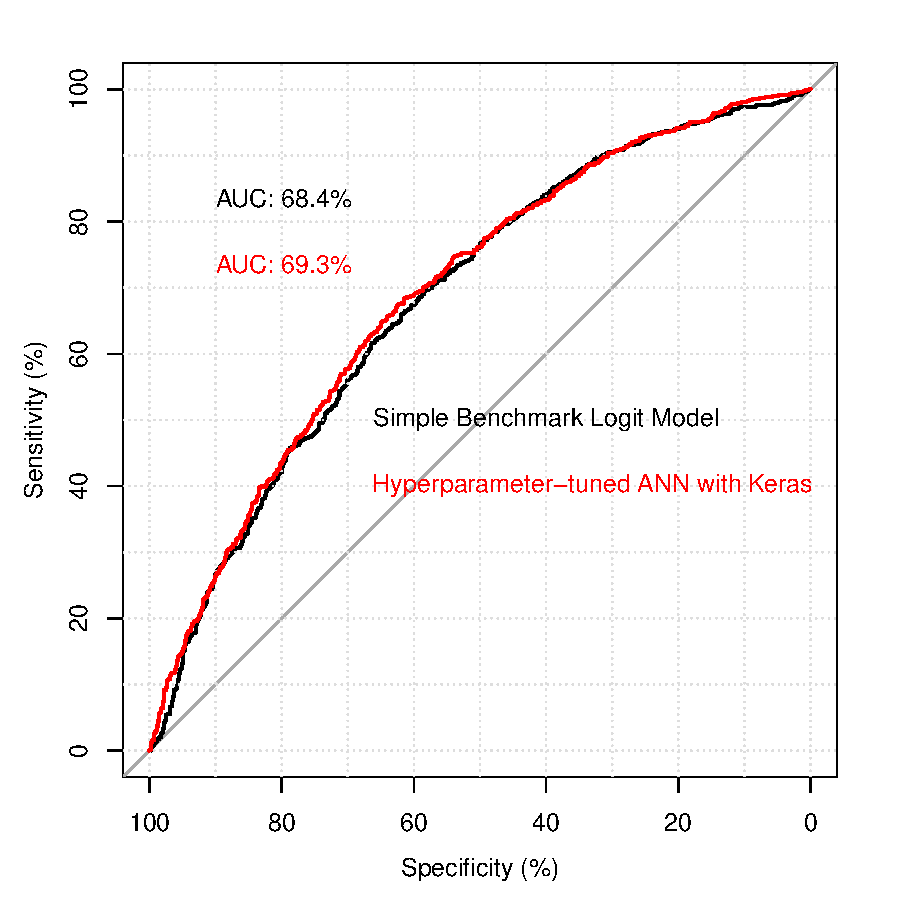
\includegraphics[scale=0.63]{figures/roc_auc_comp.pdf}
	\caption{ROC curve comparison between benchmark logit (black) and hyperparameter-tuned neural network predictions (red)}
	\label{fig_roc}
\end{figure}


\subsection{Beyond the Black Box: Feature Importance with LIME}
The previous section introduced the implemented ANN model specification and reported the results in terms of predictive performance.
However, prediction is only one part of the research question.
The other equally important question to address is explainability.
Out-of-the-box, machine learning algorithms such as ANN are indeed a "black-box" and thus it is impossible to understand why the model predicted which outcome.
LIME, as introduced theoretically in section \ref{sec_lime_theory}, provides insights into the reasoning of why the model came to a certain
conclusion by locally fitting an explainable model and reporting the resulting feature weights as a measure for its contribution to the prediction \citep{ribeiroWhyShouldTrust2016a}.
In this paper, I focus on explanations for individual observations, i.e. individual customers.
Explaining feature importance on a global level would be the next step.
However, the limited scope of this paper does not permit a thorough discussion of both.
In a business setting, it is crucial to understand why the model predicted a certain outcome for cross-selling of an individual customer, especially for building human trust in the machine learning algorithm's prediction \citep{ribeiroWhyShouldTrust2016a}.
The remainder of this section therefore focuses on this explanation only.

\begin{figure}[ht]
	\centering
  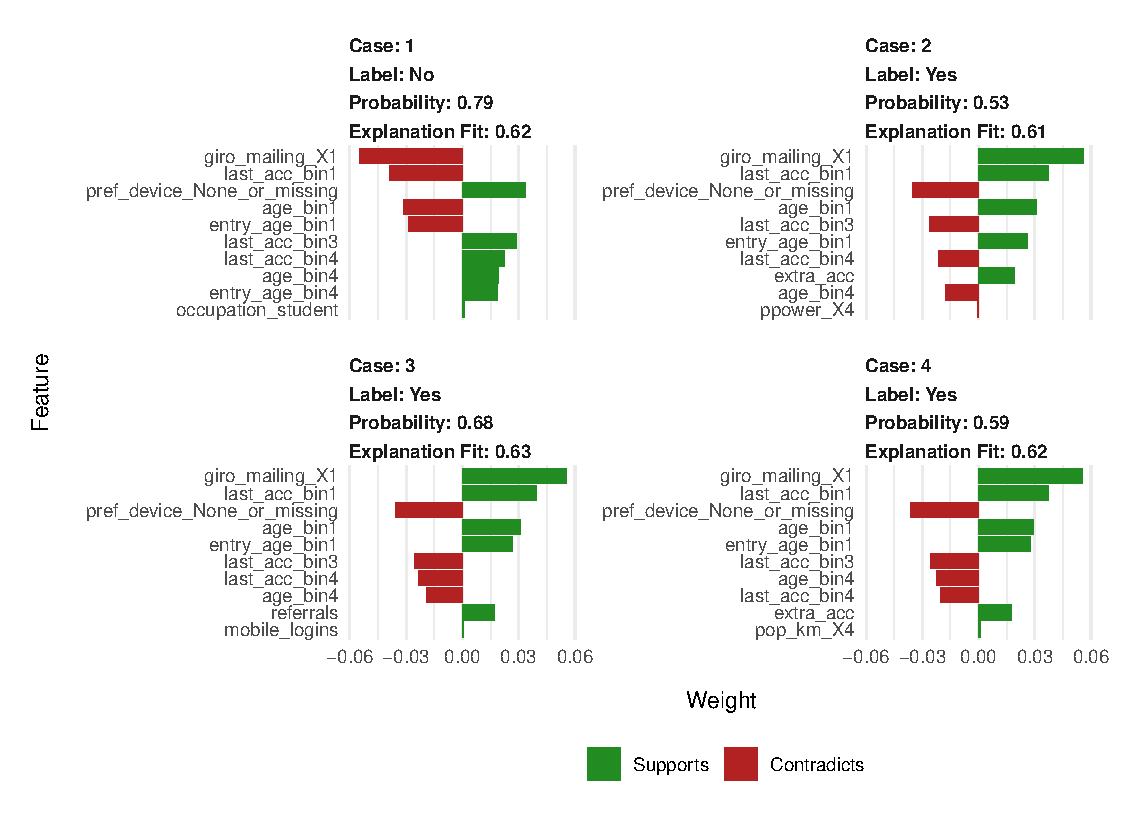
\includegraphics[scale=0.83]{figures/lime_first_four.pdf}
	\caption{LIME feature importance of the ten most important features for each of the first four customers in the test data set}
	\label{fig_lime_four}
\end{figure}

Figure \ref{fig_lime_four} visualizes the results of \pkg{lime}\code{::explain()} for the first four customers in the test data set.
For each of those customers, the ten most important features are reported in descending order of their influence on the model's prediction.
$Label$ is the model's prediction whether a customer buys another product, $probability$ gives a degree of the model's confidence in the prediction,
and $explanation\ fit$ reports the locally approximated model's $R^2$ with the ten most important features utilized.
It is apparent that the features exhibiting the highest correlation with \code{xsell} also play the biggest role for those four customers 
(see figure \ref{fig_corr} in the appendix for a graphical representation of correlation in the data set). 

A red bar indicates that the particular value of this feature contradicts the model's conclusion,
while a green bar signals supporting evidence to the model's prediction.
Whether the customer received an advertisement mail about opening a checking account (\code{giro\_mailing\_X1}) shows the largest weight from the regression model in every one of the four cases.
Also the group with the lowest days passed since the customer last opened an account (\code{last\_acc\_bin1}) shows a very large contribution to the 
prediction in those four cases.
Additionally, the customers' age seems to have a big impact on cross-sell predictions---its binned version is consistently included as a top reason for the predictions.
However, note that no generalization on the entire data set is possible from this interpretation, since it only explains individual predictions.

A first step towards a general statement about the customer base's characteristics is looking at the distribution of features split by whether the customer
opened a checking account or not.
For \code{age}, the violin plot in figure \ref{fig_violin_age} shows a striking difference in the age distribution.
Younger customers tend to more often cross-buy.
Looking at the correlation of all features with \code{xsell} in figure \ref{fig_corr} in the appendix, the youngest age group shows the highest positive correlation after \code{giro\_mailing\_X1}.
Receiving a mail with an offer to buy another product in every of the four individual explanations is the feature that has the highest influence on
the model's prediction, while it also displays the highest correlation with cross-sell.
On the contradicting side, a missing preferred device displays the highest negative correlation,
while it also comes up as the third most important feature in the individual LIME explanations.
Though a mere correlation does not imply causality, it can provide a first clue about general underlying mechanism and can validate the LIME results.
Judging from the first four customers only, the locally fitted models' weights are in line with the overall correlations.

Combining the LIME explanations with the actual values for those customers would now enable to act on those results.
The following section further elaborate on this issue and discusses the managerial implications that those methods bring with.

\begin{figure}[ht]
	\centering
  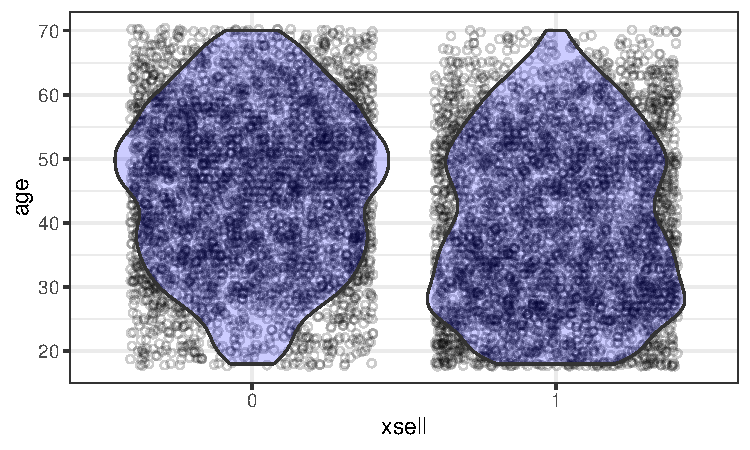
\includegraphics[scale=0.83]{figures/violin_age_xsell.pdf}
	\caption{Individual variable assessment---violin plot of xsell vs. age}
	\label{fig_violin_age}
\end{figure}

\section{Managerial and Research Implications} \label{sec_man_impl}
This section first highlights managerial implications that can be derived from this study and then outlines future research areas in this field.
Looking at the ANN's accuracy compared to a simple benchmark logit model one recommendation for practice is obvious:
Do not use neural networks in this particular business setting.
They are computationally expensive and provide no overall predictive advantage to way simpler models such as logit.
Possible reasons for the disappointing ANN performance could be the lack of enough data---neural networks require larger data sets compared
to well-specified simple regression-based models for accurately learning the underlying relationships \citep{chanClassifierDesignComputeraided1999}.
Also, neural networks are better suited for other tasks such as image recognition \citep{estevaDermatologistlevelClassificationSkin2017} and speech \citep{hintonDeepNeuralNetworks2012} or text recognition \citep{jaderbergSyntheticDataArtificial2014}.
In those cases, a simple multivariate regression would not be suitable.

Nevertheless, LIME  provides an important way to understand why the black-box ANN predicted cross-selling.
This is important to first get an understanding which features are contributing by how much and in which direction.
Out-of-the-box, this would not be possible with ANNs.
More importantly however, LIME builds trust in the prediction of an otherwise mysterious algorithm.
By fitting a locally reasonable and interpretable model, this new approach enables decision makers to assess the validity of the neural network's 
predictions beyond typical performance measures such as accuracy and AUC \citep{ribeiroWhyShouldTrust2016a}.

Still, this paper lacks a generalizeable explanation beyond simple descriptive metrics such as correlation (see figure \ref{fig_corr}) or the distribution of observations by \code{xsell} as shown in figure \ref{fig_violin_age}.
Though individual predictions can be explained by LIME, one cannot derive a truly general statement about the sample from it.
In their research on LIME, \cite{ribeiroWhyShouldTrust2016a} suggest submodular picking of individual observation-level explanations in order to 
derive generalizable insights into the black-box model.
Simplified, they propose an algorithm that optimally picks the most representative individual observations for the entire sample.
Unfortunately, the LIME-SP routine is so far only implemented in the original \proglang{Python} package and currently under development for the corresponding  \pkg{keras} \proglang{R} interface \citep{kavickyLocalInterpretableModelAgnostic2017}. 

This empirical analysis suggests which customer groups are likely to purchase another product.
Most importantly, young customers exhibit a higher probability to purchase than old ones. The more recently a customer already cross-bought,
the more likely it is that the bank can sell an additional product to this client again.
Targeting those customer groups in particular could be a valid business strategy.
However, more research would be necessary to establish a clear causal relationship between those variables.
A neural network is definitely not the method of choice for this task---even though new developments such as LIME can greatly expand the trust and explainability of black-box models.

\section{Conclusion}

The first goal of this paper was to predict whether a bank customer opens another checking account based on their individual characteristics.
A sophisticated hyper\-parameter\--tuned Artificial Neural Network was therefore introduced and its predictions compared to a simple logit model.
Surprisingly, the ANN performed slightly worse than the benchmark logit model in terms of accuracy and only marginally outperformed it in terms of AUC.
Due to the enormous computational resources required for finding a satisfactory ANN, this paper argues against the implementation of neural networks
for predicting cross-sell in this particular business setting and for simpler methods such as a logit model.

The second research question---identifying underlying characteristics that drive cross-selling---was initially impossible to answer with a black-box ANN.
However, this paper implemented a local approximation of the neural network with LIME by an easily interpretable regression model.
This enabled detailed insights into which customer features support or prevent cross-selling on an individual customer level.
Most importantly, sending mail about opening a new account is the most contributing feature for the four analyzed customers, followed directly by the customer's age.
Younger clients are more likely to cross-buy, which is also supported on the global level by looking at correlations and individual scatter plots.
Even though those two methods mostly answer the research question, there is still more research to be done to establish causality.
On a global level, the methodology implemented in this study only reports which features are associated with cross-selling.
However, no reasonable statement can be made about which features \textit{cause} an increased cross-selling probability across all customers.




\clearpage
\appendix
\section{Appendix}
\begin{figure}[ht]
	\centering
  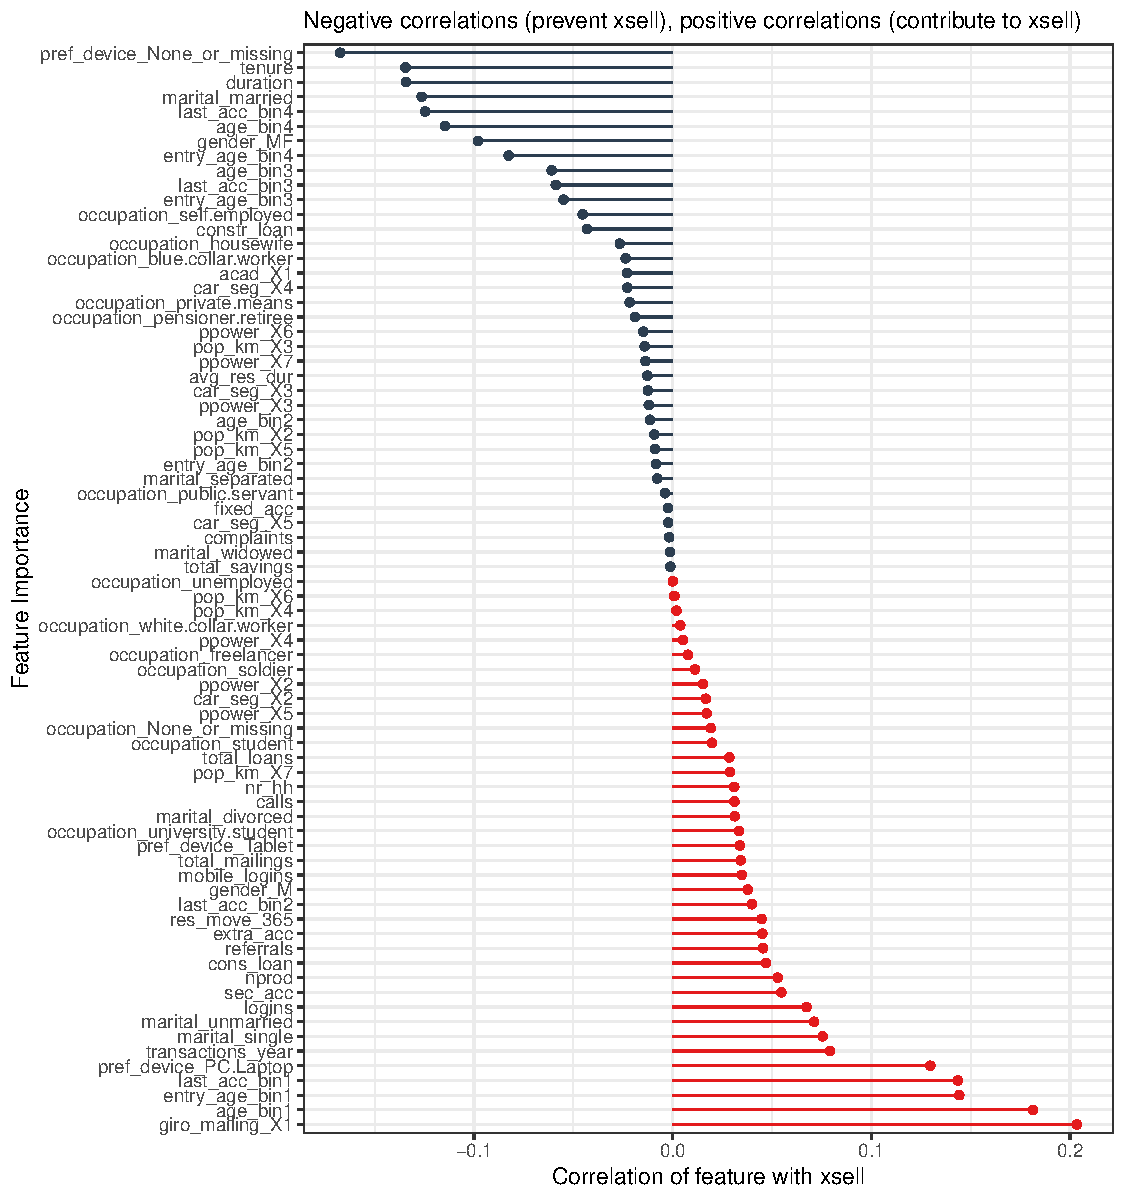
\includegraphics[scale=0.8]{figures/corrplot.pdf}
	\caption{Correlation of feature engineered variables with xsell}
	\label{fig_corr}
\end{figure}
\clearpage

\section{R Code}
\begin{lstlisting}[language=R,caption={Main analysis}, label=lst_main]
#############################################
#####             Libraries             #####
#############################################

# clear workspace
rm(list = ls())

#install packages as required

# Exception: Installing Keras is a little tricky. 
# You additionally need a python installation on your machine
#install_keras(method = "conda")

# Load libraries
library(keras)
library(lime)
library(tfruns)
library(tidyquant)
library(rsample)
library(recipes)
library(yardstick)
library(corrr)
library(randomForest)
library(missForest)
library(neuralnet)
library(caret)
library(dplyr)
library(corrplot)
library(pROC)
library(processx)
library(caret)
library(e1071)
library(stargazer)

# set same seed for R, Python, NumPy and Tensorflow
use_session_with_seed(42) 

#############################################
##  Data cleaning and Feature Engineering  ##
#############################################

# read and check data
xsell_data_raw <- read.csv("xsell.csv", na.strings=c("", "NA"), stringsAsFactors = FALSE)
glimpse(xsell_data_raw)
summary(xsell_data_raw)

# shuffle rows
xsell_data_raw <- xsell_data_raw[sample(nrow(xsell_data_raw)),]

# create new variable tenure
xsell_data_raw$tenure <- xsell_data_raw$age - xsell_data_raw$entry_age

# data cleaning, replace NAs in char-variables with "None_or_missing"
xsell_data_raw <- xsell_data_raw %>%
  replace_na(list(pref_device = "None_or_missing"))
xsell_data_raw <- xsell_data_raw %>%
  replace_na(list(occupation = "None_or_missing"))

# all character columns to factor:
xsell_data_raw <- mutate_if(xsell_data_raw, is.character, as.factor)
#additional numeric variables that should rather be treated as factors
xsell_data_raw$car_seg <- as.factor(xsell_data_raw$car_seg)
xsell_data_raw$acad <- as.factor(xsell_data_raw$acad) # remove if strange results
xsell_data_raw$giro_mailing <- as.factor(xsell_data_raw$giro_mailing) # remove if strange results
xsell_data_raw$pop_km <- as.factor(xsell_data_raw$pop_km)
xsell_data_raw$ppower <- as.factor(xsell_data_raw$ppower)

# Remove unnecessary data and clean data set
xsell_data_tbl <- xsell_data_raw %>%
  select(-X) #%>% #removes ID
  # if you don't want to run a random forest for NA imputation, you can do apply of the two easier fixes to NA's:
  #drop_na() #%>% # removes all NA's. Bad Solution! Improve! Removes 70% of observations
  #na.roughfix(xsell_data_raw) #replaces NA's: Numeric with median, factor with mode
  
# Impute NAs with a Random Forest
xsell_data_tbl$xsell <- as.factor(xsell_data_tbl$xsell) # transform to factor for random forest imputation
xsell_data_tbl <- rfImpute(xsell ~ . ,xsell_data_tbl, iter = 4, ntree=100) 
xsell_data_tbl$xsell <- as.integer(ifelse(xsell_data_tbl$xsell == "0", 0, 1)) # transform back to numeric

glimpse(xsell_data_tbl)

# Split test/training sets
train_test_split <- initial_split(xsell_data_tbl, prop = 0.8)
train_test_split

# Retrieve train and test sets
train_tbl <- training(train_test_split)
test_tbl  <- testing(train_test_split)

# define features for binning
to_bin <- c("age", "entry_age", "last_acc")

# Create recipe
rec_obj <- recipe(xsell ~ ., data = train_tbl) %>%
  step_discretize(to_bin, options = list(cuts = 4)) %>%
  step_dummy(all_nominal(), -all_outcomes()) %>%
  step_center(all_predictors(), -all_outcomes()) %>%
  step_scale(all_predictors(), -all_outcomes()) %>%
  prep(data = train_tbl)

# Apply recipe to predictors (all vars excluding xsell)
x_train_tbl <- bake(rec_obj, new_data = train_tbl) %>% select(-xsell)
x_test_tbl  <- bake(rec_obj, new_data = test_tbl) %>% select(-xsell)
glimpse(x_train_tbl)

# define response variables for training and testing sets
y_train_vec <- pull(train_tbl, xsell)
y_test_vec  <- pull(test_tbl, xsell)

# visually check transformed data set with a histogram for each feature
x_train_tbl %>% 
  gather(colnames, xsell) %>% 
  ggplot(aes(x = xsell)) + 
    geom_histogram() +
    facet_wrap(~colnames,
               scales = 'free', 
               ncol = 9)+
  theme_bw()

# correlation matrix
correl_matrix <- cor(x_train_tbl,use="pairwise.complete.obs")
# correlation plot
corrplot(correl_matrix) 

##############################################
# Building the Artificial Neural Network #####
##############################################

# I tuned the hyperparameters by trying out 324 different models
# See the scripts hyperpar_tuning_tf_runs.R and keras_nnet_architecture
# I then use the "best" hyperparameters below according to the results of those runs

# Setting up the ANN with Keras
model_keras <- keras_model_sequential()

# the hyperparameters inserted here were tuned with the hyperpar_tuning_tf_runs.R script
model_keras %>% 
  
  # First hidden layer
  layer_dense(
    units              = 64,
    kernel_initializer = "uniform", 
    activation         = "relu", 
    use_bias           = TRUE,
    bias_initializer   = 'zeros',
    input_shape        = ncol(x_train_tbl)) %>% 
  
  # Dropout to prevent overfitting
  layer_dropout(rate = 0.6) %>%

  # Second hidden layer
  layer_dense(
    units              = 128,
    kernel_initializer = "uniform",
    use_bias           = TRUE,
    bias_initializer   = 'zeros',
    activation         = "relu") %>%

 # Dropout to prevent overfitting
 layer_dropout(rate = 0.6) %>%

  # Output layer
  layer_dense(
    units              = 1, 
    kernel_initializer = "uniform", 
    activation         = "sigmoid") %>% 
  
  # Compile ANN
  compile(
    optimizer = 'adam',
    loss      = 'binary_crossentropy',
    metrics   = c('accuracy')
  )

# print model architecture
 model_keras

# Tensorboard can be useful to follow along the training of complex models as it trains
# Also, you can easily compare different models in one graph
# in this case, this is not necessary, hence commented
# launch TensorBoard (data won't show up until after the first epoch)
 
# tensorboard("logs/run_1")

history <- fit(
  object           = model_keras, 
  x                = as.matrix(x_train_tbl), 
  y                = y_train_vec,
  batch_size       = 100, 
  epochs           = 10,
  validation_split = 0.3,
  # include callback below if you want to use tensorflow
  #callbacks = callback_tensorboard("logs/run_1", write_images = TRUE),
  verbose          = 1
)

## compare runs
## In this example, I used three different callbacks for three different model specifications
# tensorboard("logs")

# Plot the training/validation history of the Keras model
plot(history) +
  theme_bw()

##############################################
## Extract Predictions from the Keras ANN ####
##############################################

# Predicted Class
yhat_keras_class_vec <- predict_classes(object = model_keras, x = as.matrix(x_test_tbl)) %>%
  as.vector()

# Predicted Class Probability
yhat_keras_prob_vec  <- predict_proba(object = model_keras, x = as.matrix(x_test_tbl)) %>%
  as.vector()


####################################################
####       Model Comparison ANN/Logit      #########
####################################################

# run script that sets up a simple benchmark Logit model
source("benchmark_logit_model.R", echo = TRUE)

# compare ANN Model ROC curve to benchmark logit modek
roc_comp <- roc(estimates_keras_tbl$truth,estimates_keras_tbl$class_prob, percent=TRUE, plot=TRUE, print.auc=TRUE,
                print.auc.x = 90, print.auc.y = 85, grid=TRUE)
roc_comp <- roc(xsell_valid$xsell,xsell_valid$pred_logit, percent=TRUE, plot=TRUE,
                 print.auc=TRUE,grid=TRUE,  col = "red", print.auc.x = 90, print.auc.y = 75, add = TRUE)
text(40,50, "Simple Benchmark Logit Model")
text(33,40, "Hyperparameter-tuned ANN with Keras", col = "red")

# compare model statistics (Confusion Matrix, Accuracy, Sensitivity, Recall, etc.)
conf_matrix_keras <- confusionMatrix(as.factor(yhat_keras_class_vec),as.factor(estimates_keras_tbl$truth), 
                             positive="1", dnn = c("Prediction", "Actual"))
conf_matrix_logit <- confusionMatrix(as.factor(xsell_valid$predict),as.factor(xsell_valid$xsell), 
                                   positive="1", dnn = c("Prediction", "Actual"))
conf_matrix_keras
conf_matrix_logit

ConfMatK <- as.data.frame.matrix(conf_matrix_keras$table)
stargazer(ConfMatK, head = FALSE, title = "Table", summary = FALSE)


####################################################
#### Evaluate Feature Importance with LIME #########
####################################################

# Setup
class(model_keras)

#Setup lime::model_type() function for keras
#This specifies that the task at hand is a classification task
model_type.keras.engine.sequential.Sequential <- function(x, ...) {
  return("classification")
  }


# Setup lime::predict_model() function for keras
predict_model.keras.engine.sequential.Sequential <- function(x, newdata, type, ...) {
  pred <- predict_proba(object = x, x = as.matrix(newdata))
  return(data.frame(Yes = pred, No = 1 - pred))
  }


# Test the predict_model() function
predict_model(x = model_keras, newdata = x_test_tbl, type = 'raw') %>%
  tibble::as_tibble()

# Run lime() on training set
explainer <- lime::lime(
  x              = x_train_tbl, 
  model          = model_keras, 
  bin_continuous = FALSE
)

# Run explain() on explainer
explanation <- lime::explain(
  x_test_tbl[1:4, ], 
  explainer      = explainer, 
  n_labels       = 1, 
  n_features     = 10,
  kernel_width   = 0.5,
  feature_select = "forward_selection"
)

# Plot feature importance
plot_features(explanation, ncol = 2) #+
  labs(title = "LIME Feature Importance Visualization",
       caption = "Test data set, first four customers")

plot_explanations(explanation) +
  labs(title = "LIME Feature Importance Heatmap",
       subtitle = "Hold Out (Test) Set, First Four Cases Shown") +
  theme_bw()

# Feature correlations to xsell
corrr_analysis <- x_train_tbl %>%
  mutate(xsell = y_train_vec) %>%
  correlate() %>%
  focus(xsell) %>%
  rename(feature = rowname) %>%
  arrange(abs(xsell)) %>%
  mutate(feature = as_factor(feature)) 

# Correlation visualization
corrr_analysis %>%
  ggplot(aes(x = xsell, y = fct_reorder(feature, desc(xsell)))) +
  geom_point() +
  # Positive Correlations - Contribute to xsell
  geom_segment(aes(xend = 0, yend = feature), 
               color = palette_light()[[2]], 
               data = corrr_analysis %>% filter(xsell > 0)) +
  geom_point(color = palette_light()[[2]], 
             data = corrr_analysis %>% filter(xsell > 0)) +
  # Negative Correlations - Prevent xsell
  geom_segment(aes(xend = 0, yend = feature), 
               color = palette_light()[[1]], 
               data = corrr_analysis %>% filter(xsell < 0)) +
  geom_point(color = palette_light()[[1]], 
             data = corrr_analysis %>% filter(xsell < 0)) +
  # Vertical lines
  # geom_vline(xintercept = 0, color = palette_light()[[5]], size = 1, linetype = 2) +
  # geom_vline(xintercept = -0.05, color = palette_light()[[5]], size = 1, linetype = 2) +
  # geom_vline(xintercept = 0.05, color = palette_light()[[5]], size = 1, linetype = 2) +
  # Aesthetics
  theme_bw() + # theme_tq replaced because in conflict with randomForest package
  labs(#title = "Cross Sell Correlation Analysis",
       subtitle = paste("Negative correlations (prevent xsell),",
                        "positive correlations (contribute to xsell)"),
       x = "Correlation of feature with xsell",
       y = "Feature Importance")

# individual variable assessment: age
train_tbl %>% 
  ggplot(aes(x=as.factor(xsell), y=age))+
  geom_jitter(shape = 1, alpha = 0.2) +
  geom_violin(fill="blue", alpha = 0.2) +
  labs(x = "xsell")+
  theme_bw()

# individual variable assessment: giro mailing
table(as.factor(train_tbl$xsell), train_tbl$giro_mailing)

# individual variable assessment: logins
train_tbl %>% 
  ggplot(aes(x=as.factor(xsell), y=logins))+
  geom_jitter(shape = 1, alpha = 0.5) +
  geom_violin(fill="blue", alpha = 0.2) +
  ylim(0,10) +
  theme_bw()

table(train_tbl$xsell, train_tbl$gender)
      
\end{lstlisting}
\begin{lstlisting}[language=R,caption={Hyperparameter tuning routine}, label=lst_tuning]
#####################################
#### Hyperparameter tuning ##########
#####################################

# run the external script with defined flags as default
training_run("keras_nnet_architecture.R")

# !!CAUTION!! Combines every single combination (3^(#tuned parameters)), thus long runtime 
# run various combinations of dropout1 and dropout2

# Only Dropout tuning
runs <- tuning_run("keras_nnet_architecture.R", runs_dir = "dropout_tuning", flags = list(
  dropout1 = c(0.2, 0.4, 0.6),
  dropout2 = c(0.2, 0.4, 0.6)
))

# run combinations of dense units, epochs and batch size
runs <- tuning_run("keras_nnet_architecture.R", runs_dir = "runs/20190608_neurons_epochs_batch_tuning", flags = list(
  #dropout1 = c(0.2, 0.4, 0.6),
  #dropout2 = c(0.2, 0.4, 0.6),
  dense_units1 = c(8, 64, 128),
  dense_units2 = c(8, 64, 128),
  epochs = c(5, 10, 30),
  batch_size = c(50, 100, 150)
))

# only number of neurons per layer tuning
runs <- tuning_run("keras_nnet_architecture.R", runs_dir = "number_neurons_tuning", flags = list(
  dense_units1 = c(8, 32, 64),
  dense_units2 = c(8, 32, 64)
))


######################################
#### After-tunig processing ##########
######################################

# check latest run
latest_run()

# compare runs in interactive RStudio viewer
compare_runs()

# View the run with the highes val_acc
view_run("runs/20190608_neurons_epochs_batch_tuning/2019-06-08T08-56-30Z")

# compare runs in data frame
runs1 <- ls_runs(runs_dir = "runs/20190607_dropout_neurons_epochs_tuning", order = metric_val_acc)
runs2 <- ls_runs(runs_dir = "runs/20190608_neurons_epochs_batch_tuning", order = metric_val_acc)

# combine both runs in one df
runs <- rbind(runs1, runs2)

# extract important information only for printing with stargazer
runs_print <- runs %>%
  arrange(desc(metric_val_acc)) %>% 
  select(metric_val_acc, metric_acc, flag_dense_units1, flag_dropout1,
         flag_dense_units2, flag_dropout2, flag_epochs, flag_batch_size)

stargazer(runs_print[1:5,], summary = FALSE)
stargazer(runs_print[323:324,], summary = FALSE)

# move all runs into run/archive
clean_runs()

# extract and save certain model
copy_run_files("runs/2019-06-08T00-38-43Z", to = "20190607-best-model")
      
\end{lstlisting}
\begin{lstlisting}[language=R,caption={Flagged neural net architecture for hyperparameter tuning}, label=lst_architecture]
##########################################
### keras neural network architecture ####
##########################################

# to be called by hyperpar_tuning_tf_runs.R

# setting up flags for hyperparameter tuning
FLAGS <- flags(
  flag_integer("dense_units1", 8),
  flag_numeric("dropout1", 0.6),
  flag_integer("dense_units2", 64),
  flag_numeric("dropout2", 0.6),
  flag_integer("epochs", 30),
  flag_integer("batch_size", 128)
)


# Setting up the ANN with Keras
model_keras <- keras_model_sequential()

model_keras %>% 
  
  # First hidden layer
  layer_dense(
    units              = FLAGS$dense_units1,
    kernel_initializer = "uniform", 
    activation         = "relu", 
    use_bias           = TRUE,
    bias_initializer   = 'zeros',
    input_shape        = ncol(x_train_tbl)) %>% 
  
  # Dropout to prevent overfitting
  layer_dropout(rate = FLAGS$dropout1) %>%
  
  # Second hidden layer
  layer_dense(
    units              = FLAGS$dense_units2,
    kernel_initializer = "uniform",
    use_bias           = TRUE,
    bias_initializer   = 'zeros',
    activation         = "relu") %>%
  
  # Dropout to prevent overfitting
  layer_dropout(rate = FLAGS$dropout2) %>%

  # Output layer
  layer_dense(
    units              = 1, 
    kernel_initializer = "uniform", 
    activation         = "sigmoid") %>% 
  
  # Compile ANN
  compile(
    optimizer = 'adam',
    loss      = 'binary_crossentropy',
    metrics   = c('accuracy')
  )


history <- fit(
  object           = model_keras, 
  x                = as.matrix(x_train_tbl), 
  y                = y_train_vec,
  batch_size       = FLAGS$batch_size, 
  epochs           = FLAGS$epochs,
  validation_split = 0.3,
  verbose          = 0
)

      
\end{lstlisting}
\begin{lstlisting}[language=R,caption={Using the ANN to predict the previously unseen out-of-time data set}, label=lst_oot]
#############################################
###   Apply model to out-of-time sample   ###
#############################################

# import oot data set
xsell_oot <- read.csv("xsell_oot.csv", na.strings=c("","NA"), stringsAsFactors = FALSE)

# create new variable tenure
xsell_oot$tenure <- xsell_oot$age - xsell_oot$entry_age

# data cleaning, replace NAs in char-variables with "None_or_missing"
xsell_oot <- xsell_oot %>%
  replace_na(list(pref_device = "None_or_missing"))
xsell_oot <- xsell_oot %>%
  replace_na(list(occupation = "None_or_missing"))

# all character columns to factor:
xsell_oot <- mutate_if(xsell_oot, is.character, as.factor)
#additional numeric variables that should rather be treated as factors
xsell_oot$car_seg <- as.factor(xsell_oot$car_seg)
xsell_oot$acad <- as.factor(xsell_oot$acad) # remove if strange results
xsell_oot$giro_mailing <- as.factor(xsell_oot$giro_mailing) # remove if strange results
xsell_oot$pop_km <- as.factor(xsell_oot$pop_km)
xsell_oot$ppower <- as.factor(xsell_oot$ppower)

# extract ID (X)
X <- xsell_oot$X

# Remove unnecessary data and clean data set
xsell_oot_data_tbl <- xsell_oot %>%
  select(-X) %>% #removes ID
  # if you don't want to run a random forest for NA imputation, you can do apply of the two easier fixes to NA's:
  #drop_na() #%>% # removes all NA's. Bad Solution! Improve! Removes 70% of observations
  na.roughfix() #replaces NA's: Numeric with median, factor with mode

# Impute NAs with a Random Forest
# can't do here, because there is no xsell
#xsell_oot_data_tbl <- rfImpute(xsell ~ . ,xsell_oot_data_tbl, iter = 4, ntree=100) 

# apply recipe to normalize, etc.
x_valid_tbl <- bake(rec_obj, new_data = xsell_oot_data_tbl)

# Predicted Class
yhat_keras_class_vec_oot <- predict_classes(object = model_keras, x = as.matrix(x_valid_tbl)) %>%
  as.vector()

xsell_oot_incl_pred <- cbind(X, xsell_pred = yhat_keras_class_vec_oot)
write.csv(xsell_oot_incl_pred, "xsell_oot_predicted.csv", row.names = FALSE)

      
\end{lstlisting}

\clearpage
\bibliography{library}

\newpage
\thispagestyle{empty}
\section*{Statutory Declaration}

Ich versichere hiermit, dass ich die vorliegende Arbeit selbs\"andig und ohne Benutzung anderer als der angegebenen Quellen und Hilfsmittel verfasst habe. W\"ortlich \"ubernommene S\"atze oder Satzteile sind als Zitat belegt, andere Anlehnungen, hinsichtlich Aussage und Umfang, unter Quellenangabe kenntlich gemacht. Die Arbeit hat in gleicher oder \"ahnlicher Form noch keiner Pr\"ufungsbeh\"orde vorgelegen und ist nicht ver\"offentlicht. Sie wurde nicht, auch nicht auszugsweise, f\"ur eine andere Pr\"ufungs- oder Studienleistung verwendet.


I herewith declare that I have completed the present term paper independently, without making use of
other than the specified literature and aids. Sentences or parts of sentences quoted literally are
marked as quotations; identification of other references with regard to the statement and scope of
the work is quoted. The thesis in this form or in any other form has not been submitted to an examination body and has not been published.
This thesis has not been used, either in whole or part, for another examination achievement.

\vspace{1cm}

Frankfurt am Main, July 15, 2019

\includegraphics[scale=0.12]{signature.png}\\
Lukas J\"urgensmeier
\end{document}
